\setcounter{section}{95}
\section{Задача LCA. Постановка, решение с помощью двоичных подъёмов. }

\begin{figure}[!htb]
   \begin{minipage}{.5\textwidth}
     \centering
     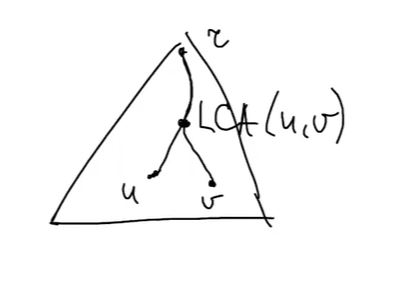
\includegraphics[height = 2 cm]{images/96-99_lca2}
     \caption{Пример задачи LCA.}
   \end{minipage}\hfill
    \begin{minipage}{.5\textwidth}
     \centering
     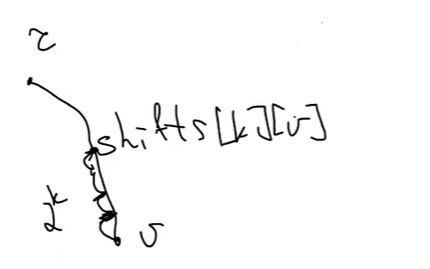
\includegraphics[height = 2 cm]{images/96-99_shifts}
     \caption{Бинарные подъёмы.}
   \end{minipage}
\end{figure}

\textbf{Задача LCA - Least (lowest) Common Ancestor}. Предком назовём путь от корня к данному узлу, тогда возникает задача найти самого низко расположенного общего предка для двух вершин в фиксированном дереве, подвешенном за корень r.

1. Разберёмся, как проверять, является ли одна вершина предком другой (u является предком самой себя).

\lstinputlisting[language=C++, emph={int,char,double,float,unsigned,vector,<,>,map}, emphstyle={\color{blue}} ]{code/96-99_ancestor.cpp}

2. Бинарные подъёмы: shifts[k][v] - предок в поколении $2^k$ для вершины v (или корень, если k слишком большой) - см. рис. 2.

shift[0][v] = parent[v];
Пусть shifts[k][v] = p, тогда shifts[k+1][v] = shifts[k][p].

Тогда вся таблица обсчитывается за $O(n log(n))$, так как $k \leqslant log(n)$.

3. Пишем алгоритм поиска LCA:

\lstinputlisting[language=C++, emph={int,char,double,float,unsigned,vector,<,>,map}, emphstyle={\color{blue}} ]{code/96-99_lca.cpp}

Асимптотика: предпосчёт $O(n log(n)$, шаг 3 - $O(log (n))$
\newpage

\setcounter{section}{96}
\section{Задача LCA. Решение с помощью эйлерова обхода. }

\begin{figure}[!htb]
   \begin{minipage}{\textwidth}
     \centering
     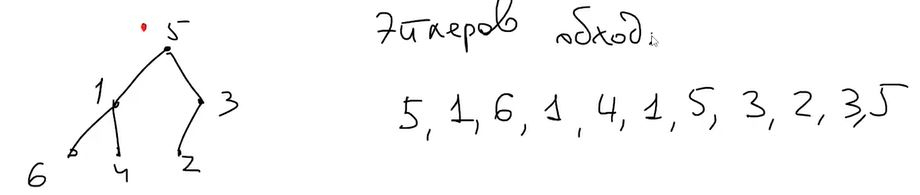
\includegraphics[height = 2 cm]{images/96-99_euler}
     \caption{Пример эйлерова обхода.}
   \end{minipage}\hfill
\end{figure}

Также задачу LCA можно решить с помощью Sparse Table на эйлеровом обходе.

Эйлеров обход - печатает вершины в том порядке, в котором мы встречаем их в dfs. Тезис: между первыми вхождениями u и v в эйлеров обход встретится lca, при том какой-то более высокий общий предок не встретится.

Вывод: осталось найти вершину с минимальной глубиной из тех, которые перечислены между вхождениями u и v.

Длина эйлерова обхода: $O(n)$. Тогда на нём можно построить SparseTable на глубинах - предпосчёт за $O(n log(n))$, ответ на запрос за $O(1)$ (стало чуть лучше, чем предыдущий алгоритм, в силу скорости ответа на запрос).

\setcounter{section}{97}
\section{Задача LCA. Алгоритм Фарах-Колтона и Бендера.}

Решает задачу LCA: предпосчёт за $O(n)$, запрос за $O(1)$.

Пользуемся предыдущим билетом: свели задачу LCA к поиску минимума на отрезке \textit{(Range-Minimum Query, RMQ)}. Но этот RMQ специфический в силу того, что у нас соседние элементы отличаются на единицу.

\textbf{Алгоритм}. 

0. Пусть есть массив длины n. Фиксируем $k = \frac{1}{2} log_2(n)$ + разобьём массив на блоки длины k. Тогда можно будет брать минимум по блокам и/или их префиксам/суффиксам.

Возьмём блок длины k, который начинается с нуля - \textbf{нормализованный}. Всего возможных нормализованных блоков - $2^{k-1} = O(\sqrt{n})$, так как на каждом следующем из k-1 элементов мы либо делаем +1, либо делаем -1 относительно предыдущего элемента, а первый у нас фиксирован.

1. Делаем все блоки нормализованными (вычитаем первый элемент), запоминаем, что вычли.

2. Кодируем каждый нормализованный блок int'ом или long long'ом.

3. Для всех нормализованных блоков находим минимумы на всех префиксах/суффиксах. Время: $O(\sqrt(n) log(n))$

4. Строим Sparse Table на $\frac{n}{k}$ блоков, где вместо блока пишем минимум на этом блоке. Время: $O(\frac{n}{k} log(\frac{n}{k})) = O(\frac{n}{log(n)} log(\frac{n}{log(n)})) = O(n - \frac{nlog(log(n))}{log(n)}) = O(n)$.

Ответ считаем за O(1): у нас закодированы наши нормализованные блоки, по коду мы находим минимумы на префиксах/суффиксах + на каждом из внутренних блоков (которые входят в отрезок полностью), выбираем самый минимальный минимум на всех (на внутренних - поиск минимума по отрезкам SparseTable, работает за O(1), +2 минимума на концах (суффикс + префикс)).

Предпосчёт: смотрим 3 и 4 пункты, слагаемое из 4 пункта превалирует, получается $O(n)$.

\newpage

\setcounter{section}{98}
\section{Задача RMQ. Постановка, решение за O(n) предподсчёта и O(1) на запрос.}

\begin{figure}[!htb]
   \begin{minipage}{.5\textwidth}
     \centering
     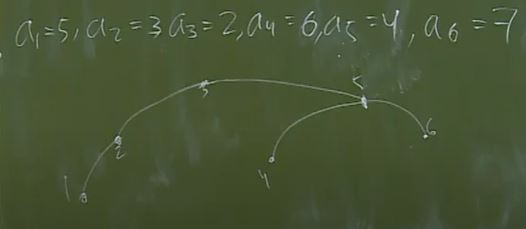
\includegraphics[height = 3 cm]{images/96-99_rmq}
     \caption{Пример графа, который мы строим}
   \end{minipage}\hfill
    \begin{minipage}{.5\textwidth}
     \centering
     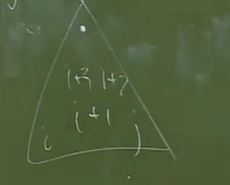
\includegraphics[height = 3 cm]{images/96-99_rmq2}
     \caption{Сплит по i, j}
   \end{minipage}
\end{figure}

\textbf{RMQ (Range-Minimum Query)} - задача о поиске минимума на подотрезке. \textbf{Попробуем решить произвольный RMQ за то же время, сведя RMQ к LCA и воспользовавшись алгоритмом Фарах-Колтона.}

Пусть у нас массив $a_1a_2 \dots a_n$, и в нём надо научиться находить минимум на отрезке. Рассмотрим декартово дерево на наборе точек: $(1, a_1), (2, a_2), \dots, (n, a_n)$ (т.е. ключ - порядок, а приоритет - наши элементы, см. рис. 4). Чтобы найти минимум на отрезке с i по j, надо найти LCA в таком декартовом дереве, и оно будет соответствовать минимальному среди этих значений. 

\textbf{Утверждение}. Если $(k, a_k)$ - LCA точек $(i, a_i)$ и $(j, a_j)$, то $a_k = min(a_i, a_{i+1}, \dots, a_j)$.

$\blacktriangle$
Сделаем split по ключам $\leqslant j$ и $\geqslant i$ - это все ключи в отрезке от i до j. (см. рис. 5 - выделенная точка - искомый минимум). 

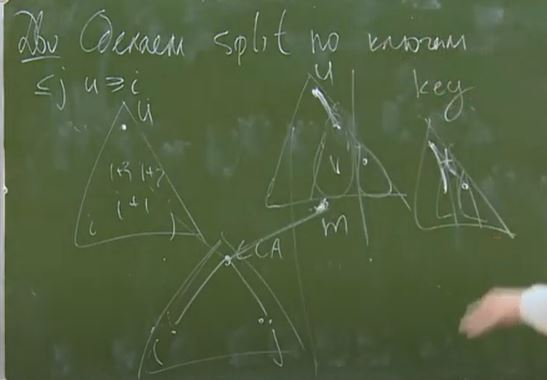
\includegraphics[]{images/96-99_split}

Вспоминаем, как работает split: идея с переподвешиваниями. В терминах рёбер меняется только "перекладывание" слева направо, т.е. выделенная вершина как была предком v, так и осталась. Тогда, по сути, в контексте split новые рёбра не появляются, они только пропадают (вместе с вершинами), поэтому не может быть такого, что какая-то вершина станет предком своего бывшего предка. Корень в поддереве в исходном дереве был минимумом (и предком i, j), и в новом дереве он всё ещё общий предок i, j.

Осталось доказать, что в сплит не попадают вершины, которые являются более старшими предками, чем LCA, т.е., что равносильно, i и j лежат в разных поддеревьях относительно корня.
$\blacksquare$

Split мы не делаем в декартовом дереве, мы исключительно ищем LCA, сплит нужен для доказательства, так что нам осталось лишь научиться строить декартово дерево за линию.

Пусть построено дерево для элементов с ключами от 1 до k. К нам пришёл новый ключ, значит, он располагается правее, дальше сравниваем его положение по вертикали и перепривязываем элементы, как на рисунке.

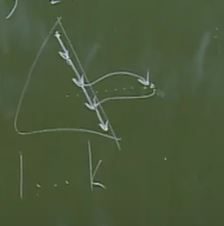
\includegraphics[height = 4 cm]{images/96-99_decart}

Таким образом, достаточно хранить правую ветку в виде стека: удаляем несколько элементов, пока не дойдём до нужного, и там перепривязываем (+ добавляем в стек).